\documentclass{beamer}
%\usepackage[T1]{fontenc}
\usepackage[utf8]{inputenc}
%\usepackage{lmodern}  % Use the Latin Modern font family

\usepackage{latexsym,amsmath,xcolor,bm, amssymb, color, tikz, graphicx, amsthm, mathtools}
\usepackage{algorithm}
\usepackage{algorithmic}
\usepackage{hyperref}
\usepackage{float}
\usepackage{multicol}

\graphicspath{{../logos/}}

\DeclareMathOperator*{\argmax}{arg\,max}
\DeclareMathOperator*{\argmin}{arg\,min}
\DeclareMathOperator{\sign}{sign}
\DeclareMathOperator{\Tr}{Tr}

\makeatletter
\DeclareRobustCommand\onedot{\futurelet\@let@token\@onedot}
\def\@onedot{\ifx\@let@token.\else.\null\fi\xspace}
\def\eg{\emph{e.g}\onedot} 
\def\Eg{\emph{E.g}\onedot}
\def\ie{\emph{i.e}\onedot} 
\def\Ie{\emph{I.e}\onedot}
\def\cf{\emph{c.f}\onedot} 
\def\Cf{\emph{C.f}\onedot}
\def\etc{\emph{etc}\onedot} 
\def\vs{\emph{vs}\onedot}
\def\wrt{w.r.t\onedot} 
\def\dof{d.o.f\onedot}
\def\etal{\emph{et al}\onedot}
\makeatother


\usetheme{Madrid}
\useinnertheme{circles}


\definecolor{ColorUNLP}{HTML}{8c0011} 
\usecolortheme[named=ColorUNLP]{structure}
%\usecolortheme[named=ColorUNR]{exampleblock}

%\setbeamertemplate{blocks}[rounded][shadow=true]
%\setbeamercolor{block body}{fg=black,bg=white}



%------------------------------------------------------------
%This block of code defines the information to appear in the
%Title page
\title %optional
{Estructuras de Datos}

\subtitle{Inicial}

%\subtitle{with applications to persuation and lie production}
% \author % (optional)
% {Author Name}

\author[Mariano Feresin]{Mariano Feresin}

\institute[]{Universidad Nacional de La Plata – Facultad de Informática}
\date[TC 2026]{Training Camp 2026}
\titlegraphic{
\includegraphics[clip,height=2cm,keepaspectratio]{logoTC.pdf}}

%End of title page configuration block
%------------------------------------------------------------


%------------------------------------------------------------
% \AtBeginSection inserts an automatic Outline slide at the start of
% each \section{}, highlighting the current section. Change the
% \section names below to your real topic names and these slides
% will update automatically.
\AtBeginSection[]
{
  \begin{frame}
    \frametitle{Outline}
    \tableofcontents[currentsection]
  \end{frame}
}
%------------------------------------------------------------


\begin{document}


%The next statement creates the title page.
\frame{\titlepage}


%------------------------------------------------------------
% Frame de Sponsors, me parece mejor ponerlo al principio
% Antes del índice/contenido

% --- Organizadores y Sponsors ---
\begin{frame}{Gracias Sponsors!}
    \begin{columns}[t]
        \column{0.5\textwidth}
        \centering
        Organiza\\
        \vspace{0.5cm}
        
\includegraphics[width=0.6\textwidth,keepaspectratio]{logo_aapc.png}\\
        \vspace{0.3cm}
        
\includegraphics[width=0.8\textwidth,keepaspectratio]{unlp_informatica.png}
        \column{0.5\textwidth}
        \centering
        Diamond Sponsor\\
        \vspace{0.5cm}
        
\includegraphics[width=0.8\textwidth,keepaspectratio]{GTSlogo.jpeg}
    \end{columns}
\end{frame}


%---------------------------------------------------------
%This block of code is for the table of contents after
%the title page
\begin{frame}
\frametitle{Outline}
\tableofcontents
\end{frame}
%---------------------------------------------------------


% ============================================================
% Introducción
% ============================================================
\section{Introducción}

\begin{frame}{Para empezar, algunas preguntas}
    \begin{itemize}
        \item ¿Para qué usamos estructuras de datos?
        \item ¿Por qué no metemos todo en un array?
        \item ¿Qué ventajas ganamos? ¿Velocidad de acceso? ¿De búsqueda?
        \item ¿Qué desventajas? ¿Más memoria?
    \end{itemize}
\end{frame}


\begin{frame}{¿Qué es una estructura de datos?}
    Con los datos de un problema siempre hacemos lo mismo:
    guardarlos, consultarlos y modificarlos.

    \vspace{0.3cm}
    \begin{block}{Idea central}
        Una estructura de datos es una forma de \textbf{organizar} los datos
        para que ciertas operaciones sean \textbf{rápidas}.
    \end{block}
\end{frame}


\begin{frame}{¿Por qué no metemos todo en un array?}
    \textbf{¡Podemos!} El array soporta todas las operaciones\ldots{}
    pero cada una tiene un costo.
    \begin{table}
        \centering
        \begin{tabular}{|l|c|}
            \hline
            \textbf{Operación (array de $N$ elementos)} & \textbf{Costo} \\
            \hline
            Acceder por posición & $\mathcal{O}(1)$ \\
            Agregar al final & $\mathcal{O}(1)$ \\
            Buscar un elemento & $\mathcal{O}(N)$ \\
            Insertar / borrar al principio & $\mathcal{O}(N)$ \\
            Encontrar el mínimo & $\mathcal{O}(N)$ \\
            \hline
        \end{tabular}
    \end{table}
    \vspace{0.2cm}
    El array no es ``malo'': es rapidísimo en algunas operaciones
    y lento en otras.
\end{frame}


\begin{frame}{Ventajas y desventajas: no hay magia}
    \textbf{Toda estructura hace un intercambio (\textit{trade-off}):}
    gana velocidad en algunas operaciones a cambio de\ldots
    \begin{itemize}
        \item usar \textbf{más memoria} (punteros, nodos, espacio extra),
        \item hacer \textbf{otras operaciones más lentas}, o directamente no soportarlas,
        \item a veces perder cosas, como el orden de inserción.
    \end{itemize}
    \vspace{0.3cm}
    No existe la estructura ``mejor en todo'':
    si existiera, usaríamos siempre esa.
\end{frame}


\begin{frame}{La pregunta clave}
    \begin{alertblock}{Cada vez que veamos una estructura, preguntarse:}
        \centering
        ¿Qué operaciones son \textbf{eficientes} en esta estructura de datos?
    \end{alertblock}
    \vspace{0.3cm}
    \textbf{Receta para elegir estructura:}
    \begin{enumerate}
        \item Listar las operaciones que necesita mi solución.
        \item Contar cuántas veces se ejecuta cada una.
        \item Elegir la estructura donde las operaciones frecuentes sean baratas.
    \end{enumerate}
    \vspace{0.3cm}
    En el resto de la clase vamos a recorrer las estructuras más usadas y,
    para cada una, responder siempre esta misma pregunta.
\end{frame}

% ============================================================
% Range Queries (CP Handbook, cap. 9)
% ============================================================
\section{Range Queries}

\begin{frame}{¿Qué es una range query?}
    En una \textbf{range query} nos piden calcular un valor sobre un
    \textbf{rango} $[a,b]$ de un array:
    \begin{itemize}
        \item $\texttt{sum}_q(a,b)$: la suma de los valores del rango $[a,b]$.
        \item $\texttt{min}_q(a,b)$: el mínimo del rango $[a,b]$.
        \item $\texttt{max}_q(a,b)$: el máximo del rango $[a,b]$.
    \end{itemize}

    \vspace{0.2cm}
    Por ejemplo, para el rango $[3,6]$:
    \begin{center}
    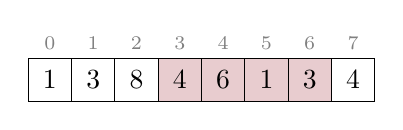
\begin{tikzpicture}[x=0.55cm, y=0.55cm]
        \fill[ColorUNLP!20] (2.5,-0.5) rectangle (6.5,0.5);
        \foreach \v [count=\i from 0] in {1,3,8,4,6,1,3,4} {
            \draw (\i-0.5,-0.5) rectangle (\i+0.5,0.5);
            \node at (\i,0) {\v};
            \node[gray] at (\i,0.85) {\scriptsize \i};
        }
    \end{tikzpicture}
    \end{center}

    \vspace{0.1cm}
    $\texttt{sum}_q(3,6)=14$, \quad $\texttt{min}_q(3,6)=1$, \quad $\texttt{max}_q(3,6)=6$.
\end{frame}


\begin{frame}[fragile]{La solución directa}
    \begin{block}{Recorrer el rango}
    \begin{verbatim}
int sum(int a, int b) {
    int s = 0;
    for (int i = a; i <= b; i++) {
        s += array[i];
    }
    return s;
}
    \end{verbatim}
    \end{block}

    \vspace{0.2cm}
    Cada consulta cuesta $\mathcal{O}(n)$. Con $q$ consultas: $\mathcal{O}(n \cdot q)$.

    \vspace{0.2cm}
    \textbf{¿Y si $n, q \leq 10^5$?} $\quad 10^5 \cdot 10^5 = 10^{10}$
    $\Rightarrow$ \textcolor{red}{no entra en tiempo}.

    \vspace{0.2cm}
    \textbf{¿Podemos responder una consulta sin recorrer todo el rango?}
\end{frame}


\begin{frame}{Arrays estáticos: prefix sums}
    Si el array \textbf{no cambia} entre consultas, podemos \textbf{precalcular}.

    \vspace{0.2cm}
    \textbf{Prefix sum array:} en la posición $k$ guardamos
    $\texttt{sum}_q(0,k)$, la suma de todo el array hasta $k$:
    \begin{center}
    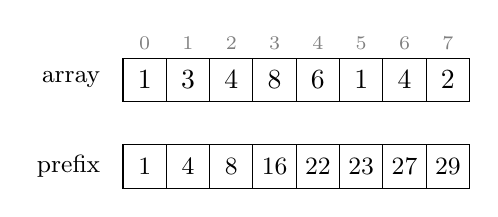
\begin{tikzpicture}[x=0.55cm, y=0.55cm]
        \node[anchor=east] at (-0.8,0) {\small array};
        \foreach \v [count=\i from 0] in {1,3,4,8,6,1,4,2} {
            \draw (\i-0.5,-0.5) rectangle (\i+0.5,0.5);
            \node at (\i,0) {\v};
            \node[gray] at (\i,0.85) {\scriptsize \i};
        }
        \node[anchor=east] at (-0.8,-2) {\small prefix};
        \foreach \v [count=\i from 0] in {1,4,8,16,22,23,27,29} {
            \draw (\i-0.5,-2.5) rectangle (\i+0.5,-1.5);
            \node at (\i,-2) {\small \v};
        }
    \end{tikzpicture}
    \end{center}

    \vspace{0.2cm}
    Se construye en $\mathcal{O}(n)$ con una sola pasada:
    $\texttt{prefix}[i] = \texttt{prefix}[i-1] + \texttt{array}[i]$.
\end{frame}


\begin{frame}[fragile]{Prefix sums: consultas en $\mathcal{O}(1)$}
    La suma de un rango es una \textbf{resta de dos prefijos}:
    \begin{center}
        $\texttt{sum}_q(a,b) = \texttt{prefix}[b] - \texttt{prefix}[a-1]$
    \end{center}

    Por ejemplo:
    $\texttt{sum}_q(3,6) = \texttt{prefix}[6] - \texttt{prefix}[2] = 27 - 8 = 19$.

    \begin{block}{Código C++}
    \begin{verbatim}
int sum(int a, int b) {
    if (a == 0) return prefix[b];
    return prefix[b] - prefix[a-1];
}
    \end{verbatim}
    \end{block}

    Construimos \textbf{una sola vez} en $\mathcal{O}(n)$, y después cada
    consulta sale en $\mathcal{O}(1)$.
\end{frame}


\begin{frame}{Prefix sums en 2D}
    La misma idea funciona en una matriz: precalculamos $S(X)$, la suma del
    rectángulo desde la esquina superior izquierda hasta la posición $X$.
    \begin{center}
    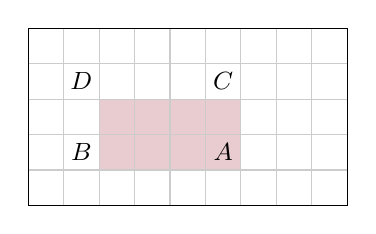
\begin{tikzpicture}[x=0.45cm, y=0.45cm]
        \fill[ColorUNLP!20] (2,1) rectangle (6,3);
        \draw[gray!40, step=1] (0,0) grid (9,5);
        \draw (0,0) rectangle (9,5);
        \node[font=\small] at (1.5,3.5) {$D$};
        \node[font=\small] at (5.5,3.5) {$C$};
        \node[font=\small] at (1.5,1.5) {$B$};
        \node[font=\small] at (5.5,1.5) {$A$};
    \end{tikzpicture}
    \end{center}

    \begin{center}
        suma del rectángulo gris $= S(A) - S(B) - S(C) + S(D)$
    \end{center}

    Cada consulta rectangular también sale en $\mathcal{O}(1)$.
\end{frame}


% --- Sparse table: fuera del temario por ahora ---
% Para reincorporar estas dos diapos, borrar el \iffalse y el \fi.
\iffalse
\begin{frame}{¿Y el mínimo? Sparse table}
    \textbf{¿Sirve el mismo truco para $\texttt{min}_q$?} No: el mínimo de un
    rango no se obtiene ``restando'' dos prefijos.

    \vspace{0.2cm}
    \textbf{Idea:} precalcular $\texttt{min}_q(a,b)$ para todos los rangos cuyo
    largo es una \textbf{potencia de 2} (1, 2, 4, 8, \ldots).
    \begin{itemize}
        \item Hay $\mathcal{O}(\log n)$ largos posibles $\Rightarrow$
              $\mathcal{O}(n \log n)$ valores precalculados.
        \item Cada valor se arma con dos mitades ya calculadas:
              rangos de largo $2w$ = dos rangos de largo $w$.
    \end{itemize}

    \vspace{0.2cm}
    Construcción: $\mathcal{O}(n \log n)$. Esta estructura se llama
    \textbf{sparse table}.
\end{frame}


\begin{frame}{Sparse table: consultas en $\mathcal{O}(1)$}
    Todo rango se cubre con \textbf{dos} rangos de largo potencia de 2 que se
    \textbf{superponen} ($k$ = mayor potencia de 2 $\leq$ largo del rango):
    \begin{center}
        $\texttt{min}_q(a,b) = \min(\texttt{min}_q(a,a+k-1),\; \texttt{min}_q(b-k+1,b))$
    \end{center}

    Ejemplo con $[1,6]$: largo 6, $k=4$ $\Rightarrow$ $[1,4] \cup [3,6]$:
    \begin{center}
    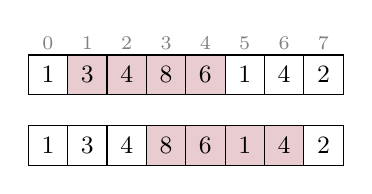
\begin{tikzpicture}[x=0.5cm, y=0.5cm]
        \fill[ColorUNLP!20] (0.5,-0.5) rectangle (4.5,0.5);
        \foreach \v [count=\i from 0] in {1,3,4,8,6,1,4,2} {
            \draw (\i-0.5,-0.5) rectangle (\i+0.5,0.5);
            \node at (\i,0) {\small \v};
            \node[gray] at (\i,0.8) {\scriptsize \i};
        }
        \fill[ColorUNLP!20] (2.5,-2.3) rectangle (6.5,-1.3);
        \foreach \v [count=\i from 0] in {1,3,4,8,6,1,4,2} {
            \draw (\i-0.5,-2.3) rectangle (\i+0.5,-1.3);
            \node at (\i,-1.8) {\small \v};
        }
    \end{tikzpicture}
    \end{center}

    $\texttt{min}_q(1,6) = \min(3, 1) = 1$. Repetir elementos
    \textbf{no molesta}: contar algo dos veces no cambia el mínimo.
\end{frame}
\fi


\begin{frame}{¿Y si el array cambia?}
    Hasta acá el array era \textbf{estático}. \textbf{¿Qué pasa si entre
    consultas nos piden actualizar un valor?}
    \begin{itemize}
        \item Array solo: update $\mathcal{O}(1)$, pero consulta $\mathcal{O}(n)$.
        \item Prefix sums: consulta $\mathcal{O}(1)$, pero cada update obliga
              a reconstruir todo: $\mathcal{O}(n)$.
    \end{itemize}

    \vspace{0.2cm}
    Con $n$ y $q$ grandes, cualquiera de las dos opciones explota.

    \vspace{0.2cm}
    \begin{alertblock}{La pregunta clave, otra vez}
        Necesitamos una estructura donde \textbf{consulta y update} sean
        eficientes \textbf{a la vez}.
    \end{alertblock}
\end{frame}


\begin{frame}{Segment tree}
    La estructura clásica para tener \textbf{consulta y update eficientes a
    la vez} es el \textbf{segment tree}:
    \begin{itemize}
        \item Árbol binario: las hojas son los elementos del array.
        \item Cada nodo interno resume su rango (suma, mín, máx, gcd, \ldots).
        \item Consulta y update en $\mathcal{O}(\log n)$.
    \end{itemize}
    \begin{center}
    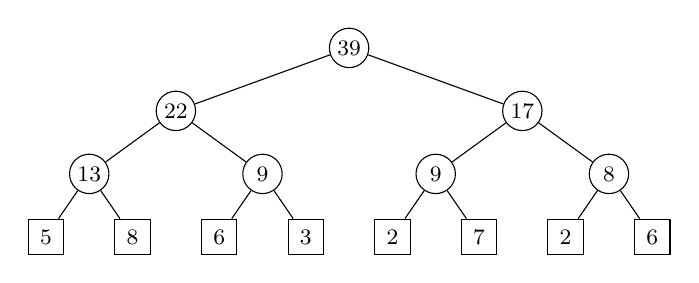
\begin{tikzpicture}[
        level distance=0.8cm,
        level 1/.style={sibling distance=4.4cm},
        level 2/.style={sibling distance=2.2cm},
        level 3/.style={sibling distance=1.1cm},
        every node/.style={circle, draw, inner sep=1pt, minimum size=0.5cm, font=\footnotesize},
        leaf/.style={rectangle, minimum size=0.45cm}]
        \node {39}
            child {node {22}
                child {node {13} child {node[leaf] {5}} child {node[leaf] {8}}}
                child {node {9} child {node[leaf] {6}} child {node[leaf] {3}}}}
            child {node {17}
                child {node {9} child {node[leaf] {2}} child {node[leaf] {7}}}
                child {node {8} child {node[leaf] {2}} child {node[leaf] {6}}}};
    \end{tikzpicture}
    \end{center}
\end{frame}


\begin{frame}{Segment tree: consulta y update en $\mathcal{O}(\log n)$}
    \textbf{Consulta:} todo rango se cubre con $\mathcal{O}(\log n)$ nodos
    (a lo sumo 2 por nivel). Por ejemplo, $\texttt{sum}_q(2,7) = 9 + 17 = 26$:
    \begin{center}
    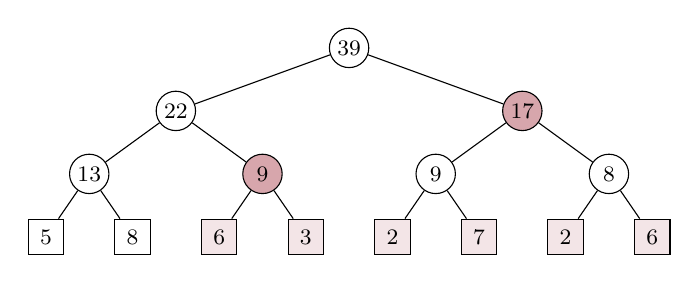
\begin{tikzpicture}[
        level distance=0.8cm,
        level 1/.style={sibling distance=4.4cm},
        level 2/.style={sibling distance=2.2cm},
        level 3/.style={sibling distance=1.1cm},
        every node/.style={circle, draw, inner sep=1pt, minimum size=0.5cm, font=\footnotesize},
        leaf/.style={rectangle, minimum size=0.45cm}]
        \node {39}
            child {node {22}
                child {node {13} child {node[leaf] {5}} child {node[leaf] {8}}}
                child {node[fill=ColorUNLP!35] {9} child {node[leaf, fill=ColorUNLP!10] {6}} child {node[leaf, fill=ColorUNLP!10] {3}}}}
            child {node[fill=ColorUNLP!35] {17}
                child {node {9} child {node[leaf, fill=ColorUNLP!10] {2}} child {node[leaf, fill=ColorUNLP!10] {7}}}
                child {node {8} child {node[leaf, fill=ColorUNLP!10] {2}} child {node[leaf, fill=ColorUNLP!10] {6}}}};
    \end{tikzpicture}
    \end{center}

    \textbf{Update:} al cambiar una hoja, solo hay que recalcular el
    \textbf{camino hasta la raíz}: $\mathcal{O}(\log n)$ nodos.
\end{frame}


\begin{frame}[fragile]{Segment tree: código}
    Se guarda en un array de $2n$ ($n$ potencia de 2): la raíz es
    $\texttt{tree}[1]$, los hijos de $\texttt{tree}[k]$ son $\texttt{tree}[2k]$
    y $\texttt{tree}[2k{+}1]$, y las hojas van de $\texttt{tree}[n]$ a
    $\texttt{tree}[2n{-}1]$.
    \begin{columns}[t]
        \column{0.52\textwidth}
        \begin{block}{Consulta: $\texttt{sum}_q(a,b)$}
        \footnotesize
\begin{verbatim}
int sum(int a, int b) {
  a += n; b += n;
  int s = 0;
  while (a <= b) {
    if (a%2 == 1) s += tree[a++];
    if (b%2 == 0) s += tree[b--];
    a /= 2; b /= 2;
  }
  return s;
}
\end{verbatim}
        \end{block}
        \column{0.44\textwidth}
        \begin{block}{Update: sumar $x$ en $k$}
        \footnotesize
\begin{verbatim}
void add(int k, int x) {
  k += n;
  tree[k] += x;
  for (k /= 2; k >= 1; k /= 2)
    tree[k] = tree[2*k]
            + tree[2*k+1];
}
\end{verbatim}
        \end{block}
    \end{columns}

    \vspace{0.1cm}
    Para mínimo: cambiar las sumas por $\min$.
\end{frame}


% --- Fenwick tree: fuera del temario por ahora (queda mencionado en
% "Otras cosas que existen"). Borrar \iffalse y \fi para reincorporar. ---
\iffalse
\begin{frame}{Fenwick tree (binary indexed tree)}
    Si \textbf{solo necesitamos sumas}, hay una alternativa al segment tree
    más corta de codear: una versión \textbf{dinámica} del prefix sum array,
    también con todo en $\mathcal{O}(\log n)$. Se indexa \textbf{desde 1}.

    \vspace{0.1cm}
    \textbf{Idea:} $\texttt{tree}[k]$ guarda la suma de un rango que
    \textbf{termina en $k$}, de largo $p(k)$ = mayor potencia de 2 que divide a $k$:
    \begin{center}
    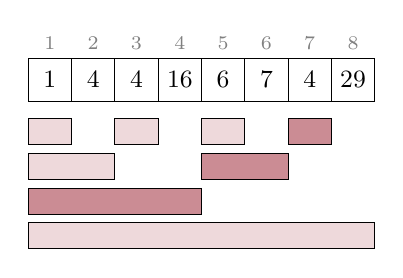
\begin{tikzpicture}[x=0.55cm, y=0.55cm]
        \foreach \v [count=\i from 1] in {1,4,4,16,6,7,4,29} {
            \draw (\i-0.5,-0.5) rectangle (\i+0.5,0.5);
            \node at (\i,0) {\small \v};
            \node[gray] at (\i,0.85) {\scriptsize \i};
        }
        \foreach \k/\a/\y in {1/1/-1.2, 3/3/-1.2, 5/5/-1.2, 2/1/-2.0, 8/1/-3.6} {
            \draw[fill=ColorUNLP!15] (\a-0.5,\y-0.3) rectangle (\k+0.5,\y+0.3);
        }
        \foreach \k/\a/\y in {7/7/-1.2, 6/5/-2.0, 4/1/-2.8} {
            \draw[fill=ColorUNLP!45] (\a-0.5,\y-0.3) rectangle (\k+0.5,\y+0.3);
        }
    \end{tikzpicture}
    \end{center}

    Todo prefijo se parte en $\mathcal{O}(\log n)$ de esos rangos. Por ejemplo:
    $\texttt{sum}_q(1,7) = \texttt{tree}[4] + \texttt{tree}[6] + \texttt{tree}[7]
    = 16 + 7 + 4 = 27$.
\end{frame}


\begin{frame}[fragile]{Fenwick tree: código}
    Magia de bits: $p(k) = \texttt{k \& -k}$.
    \begin{columns}[t]
        \column{0.48\textwidth}
        \begin{block}{Consulta: suma de $[1,k]$}
\begin{verbatim}
int sum(int k) {
    int s = 0;
    while (k >= 1) {
        s += tree[k];
        k -= k&-k;
    }
    return s;
}
\end{verbatim}
        \end{block}
        \column{0.48\textwidth}
        \begin{block}{Update: sumar $x$ en $k$}
\begin{verbatim}
void add(int k, int x) {
    while (k <= n) {
        tree[k] += x;
        k += k&-k;
    }
}
\end{verbatim}
        \end{block}
    \end{columns}

    \vspace{0.2cm}
    Ambas visitan $\mathcal{O}(\log n)$ posiciones. Para rangos generales,
    igual que con prefix sums:
    $\texttt{sum}_q(a,b) = \texttt{sum}_q(1,b) - \texttt{sum}_q(1,a-1)$.
\end{frame}
\fi


\begin{frame}{Extra 1: compresión de índices}
    \textbf{¿Y si los índices son enormes?} Por ejemplo, posiciones hasta
    $10^9$: no podemos crear un array de $10^9$ elementos.

    \vspace{0.2cm}
    Si conocemos \textbf{de antemano} todos los índices que se usan, los
    reemplazamos por $1, 2, 3, \ldots$ \textbf{conservando el orden}
    (si $a < b$, entonces $c(a) < c(b)$):
    \begin{center}
        $c(8) = 1, \qquad c(555) = 2, \qquad c(10^9) = 3$
    \end{center}

    \vspace{0.2cm}
    Con los índices comprimidos ya podemos usar cualquier estructura de este
    capítulo.
\end{frame}


\begin{frame}{Extra 2: updates de rango}
    Situación inversa: \textbf{sumar $x$ a todo un rango} $[a,b]$ y consultar
    valores sueltos. \textbf{Difference array:} las diferencias entre valores
    consecutivos (el array original es su prefix sum):
    \begin{center}
    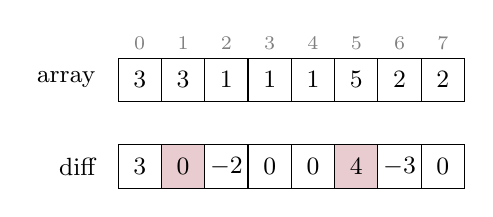
\begin{tikzpicture}[x=0.55cm, y=0.55cm]
        \node[anchor=east] at (-0.8,0) {\small array};
        \foreach \v [count=\i from 0] in {3,3,1,1,1,5,2,2} {
            \draw (\i-0.5,-0.5) rectangle (\i+0.5,0.5);
            \node at (\i,0) {\small $\v$};
            \node[gray] at (\i,0.85) {\scriptsize \i};
        }
        \node[anchor=east] at (-0.8,-2) {\small diff};
        \fill[ColorUNLP!20] (0.5,-2.5) rectangle (1.5,-1.5);
        \fill[ColorUNLP!20] (4.5,-2.5) rectangle (5.5,-1.5);
        \foreach \v [count=\i from 0] in {3,0,-2,0,0,4,-3,0} {
            \draw (\i-0.5,-2.5) rectangle (\i+0.5,-1.5);
            \node at (\i,-2) {\small $\v$};
        }
    \end{tikzpicture}
    \end{center}

    Sumar $x$ en $[a,b]$ = tocar \textbf{solo 2 posiciones}:
    $\texttt{diff}[a] \mathrel{+}= x$ y $\texttt{diff}[b+1] \mathrel{-}= x$.
    Con un segment tree sobre \texttt{diff}, todo en $\mathcal{O}(\log n)$.
\end{frame}


\begin{frame}{¿Qué estructura uso?}
    \begin{table}
        \centering
        \begin{tabular}{|l|c|c|l|}
            \hline
            \textbf{Estructura} & \textbf{Consulta} & \textbf{Update} & \textbf{Sirve para} \\
            \hline
            Prefix sums & $\mathcal{O}(1)$ & --- & sumas, estático \\
            Segment tree & $\mathcal{O}(\log n)$ & $\mathcal{O}(\log n)$ & suma, mín, máx, \ldots \\
            \hline
        \end{tabular}
    \end{table}

    \vspace{0.2cm}
    \begin{alertblock}{La pregunta clave en acción}
        ¿Qué operaciones necesita mi solución? ¿Hay updates o el array es
        estático? La respuesta elige la estructura sola.
    \end{alertblock}
\end{frame}


\begin{frame}{Otras cosas que existen (para ir a buscar)}
    Nombres para googlear cuando esta clase les quede corta:
    \begin{itemize}
        \item \textbf{Fenwick tree (BIT):} sumas con updates en
              $\mathcal{O}(\log n)$, en $\sim$10 líneas y con constante
              chica (libro, pág.~86).
        \item \textbf{Sparse table:} mín/máx en un array estático con
              consultas $\mathcal{O}(1)$ (libro, pág.~85).
        \item \textbf{Segment tree con lazy propagation:} updates a un rango
              entero \textbf{y} consultas de rango, todo en $\mathcal{O}(\log n)$.
        \item \textbf{Segment tree implícito:} índices gigantes ($10^{18}$)
              sin comprimir: los nodos se crean a medida que se usan.
        \item \textbf{Sqrt decomposition:} partir el array en bloques de
              $\sqrt{n}$; menos eficiente pero muy flexible.
        \item \textbf{Mo's algorithm:} responder muchas consultas de rango
              \textbf{offline}, reordenándolas con astucia.
    \end{itemize}
\end{frame}


\begin{frame}{Problemas para practicar (CSES)}
    \begin{itemize}
        \item \href{https://cses.fi/problemset/task/1646}{Static Range Sum Queries}
              \textcolor{white}{\scriptsize prefix sums}
        \item \href{https://cses.fi/problemset/task/1647}{Static Range Minimum Queries}
              \textcolor{white}{\scriptsize segment tree}
        \item \href{https://cses.fi/problemset/task/1648}{Dynamic Range Sum Queries}
              \textcolor{white}{\scriptsize segment tree}
        \item \href{https://cses.fi/problemset/task/1649}{Dynamic Range Minimum Queries}
              \textcolor{white}{\scriptsize segment tree}
        \item \href{https://cses.fi/problemset/task/1650}{Range Xor Queries}
              \textcolor{white}{\scriptsize prefix xor}
        \item \href{https://cses.fi/problemset/task/1651}{Range Update Queries}
              \textcolor{white}{\scriptsize difference array}
        \item \href{https://cses.fi/problemset/task/1652}{Forest Queries}
              \textcolor{white}{\scriptsize prefix sums 2D}
    \end{itemize}

    \vspace{0.2cm}
    \small (Hay pistas escritas en blanco al lado de cada problema:
    píntenlas con el mouse si se traban.)
\end{frame}


% ============================================================
% DSU / Union-Find (CP Handbook, cap. 15.3, pág. 145)
% ============================================================
\section{DSU (Union-Find)}

\begin{frame}{Problema: los grupos de la fiesta}
    En una fiesta hay $N$ personas, cada una en su propio grupo. Llegan $Q$
    eventos, de dos tipos:
    \begin{itemize}
        \item \texttt{u a b}: $a$ y $b$ se hacen amigos, y \textbf{los dos
              grupos se juntan en uno solo}.
        \item \texttt{?\ a b}: ¿están $a$ y $b$ en el \textbf{mismo grupo}?
    \end{itemize}
    con $N, Q \leq 10^5$.

    \vspace{0.3cm}
    \begin{alertblock}{Para pensar}
        \centering
        Si guardo el grupo de cada persona en un array,
        ¿cuánto cuesta \textbf{juntar} dos grupos?
    \end{alertblock}
\end{frame}


\begin{frame}{La idea: un representante por grupo}
    Guardamos una \textbf{colección de conjuntos disjuntos} (nadie está en dos
    grupos a la vez). En cada conjunto elegimos un elemento
    \textbf{representante}, y todos los demás forman una \textbf{cadena} que
    lleva hasta él.

    \vspace{0.2cm}
    \begin{center}
    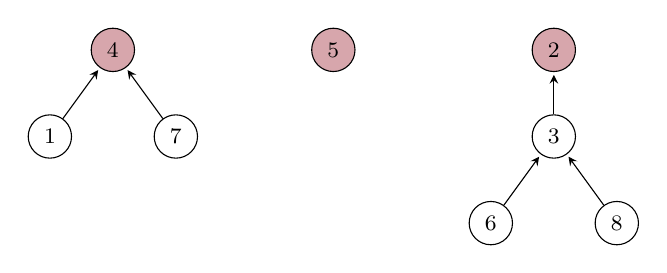
\begin{tikzpicture}[
        every node/.style={circle, draw, inner sep=1pt, minimum size=0.55cm, font=\footnotesize},
        ->, >=stealth, shorten >=1pt]
        \node[fill=ColorUNLP!35] (a4) at (0,0) {4};
        \node (a1) at (-0.8,-1.1) {1};
        \node (a7) at (0.8,-1.1) {7};
        \draw (a1) -- (a4); \draw (a7) -- (a4);

        \node[fill=ColorUNLP!35] (b5) at (2.8,0) {5};

        \node[fill=ColorUNLP!35] (c2) at (5.6,0) {2};
        \node (c3) at (5.6,-1.1) {3};
        \node (c6) at (4.8,-2.2) {6};
        \node (c8) at (6.4,-2.2) {8};
        \draw (c3) -- (c2); \draw (c6) -- (c3); \draw (c8) -- (c3);
    \end{tikzpicture}
    \end{center}

    \vspace{0.1cm}
    Acá los conjuntos son $\{1,4,7\}$, $\{5\}$ y $\{2,3,6,8\}$, con
    representantes 4, 5 y 2. Para saber el representante de 6 seguimos la
    cadena $6 \to 3 \to 2$.

    \vspace{0.1cm}
    \textbf{Dos elementos están en el mismo conjunto exactamente cuando tienen
    el mismo representante.}
\end{frame}


\begin{frame}{Unir dos conjuntos}
    Para unir dos conjuntos alcanza con \textbf{colgar el representante de uno
    del representante del otro}. Uniendo $\{1,4,7\}$ con $\{2,3,6,8\}$:

    \vspace{0.1cm}
    \begin{center}
    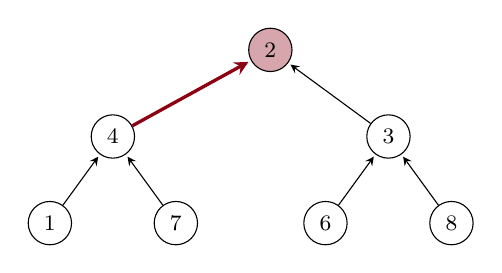
\begin{tikzpicture}[
        every node/.style={circle, draw, inner sep=1pt, minimum size=0.55cm, font=\footnotesize},
        ->, >=stealth, shorten >=1pt]
        \node[fill=ColorUNLP!35] (c2) at (0,0) {2};
        \node (a4) at (-2,-1.1) {4};
        \node (c3) at (1.5,-1.1) {3};
        \node (a1) at (-2.8,-2.2) {1};
        \node (a7) at (-1.2,-2.2) {7};
        \node (c6) at (0.7,-2.2) {6};
        \node (c8) at (2.3,-2.2) {8};
        \draw[ColorUNLP, very thick] (a4) -- (c2);
        \draw (c3) -- (c2);
        \draw (a1) -- (a4); \draw (a7) -- (a4);
        \draw (c6) -- (c3); \draw (c8) -- (c3);
    \end{tikzpicture}
    \end{center}

    \vspace{0.1cm}
    El 2 pasa a ser el representante de todo $\{1,2,3,4,6,7,8\}$, y el viejo
    representante 4 ahora apunta a 2.

    \vspace{0.2cm}
    \begin{block}{¿De cuál colgamos cuál? Unión por tamaño}
        Siempre colgamos el representante del conjunto \textbf{más chico} del
        representante del \textbf{más grande}. Así ninguna cadena se hace más
        larga que $\mathcal{O}(\log n)$.
    \end{block}
\end{frame}


\begin{frame}[fragile]{DSU: código}
    \texttt{link[x]}: el siguiente en la cadena (o \texttt{x} mismo si es
    representante). \texttt{sz[x]}: el tamaño del conjunto, solo válido en los
    representantes.
    \begin{columns}[t]
        \column{0.46\textwidth}
        \begin{block}{Inicialización}
        \footnotesize
\begin{verbatim}
for (int i = 1; i <= n; i++) {
  link[i] = i;
  sz[i] = 1;
}
\end{verbatim}
        \end{block}
        \begin{block}{find y same}
        \footnotesize
\begin{verbatim}
int find(int x) {
  while (x != link[x]) x = link[x];
  return x;
}
bool same(int a, int b) {
  return find(a) == find(b);
}
\end{verbatim}
        \end{block}
        \column{0.5\textwidth}
        \begin{block}{unite (unión por tamaño)}
        \footnotesize
\begin{verbatim}
void unite(int a, int b) {
  a = find(a);
  b = find(b);
  if (a == b) return;
  if (sz[a] < sz[b]) swap(a,b);
  sz[a] += sz[b];
  link[b] = a;
}
\end{verbatim}
        \end{block}
        \footnotesize Las tres operaciones cuestan $\mathcal{O}(\log n)$:
        lo único que hacen es recorrer una cadena.
    \end{columns}
\end{frame}


\begin{frame}[fragile]{Path compression: casi $\mathcal{O}(1)$}
    Cada vez que recorremos una cadena, la podemos \textbf{aplanar}: hacer que
    todos los nodos del camino apunten directo al representante.
    \begin{block}{find con compresión de caminos}
    \footnotesize
\begin{verbatim}
int find(int x) {
  if (x == link[x]) return x;
  return link[x] = find(link[x]);  // guarda el resultado
}
\end{verbatim}
    \end{block}

    \vspace{0.1cm}
    Es \textbf{una línea más} y no cambia el resultado: solo deja el árbol más
    chato para las próximas consultas.

    \vspace{0.2cm}
    \begin{block}{Costo}
        Con unión por tamaño \textbf{y} compresión de caminos, cada operación
        cuesta $\mathcal{O}(\alpha(n))$, donde $\alpha$ crece tan despacio que
        para cualquier $n$ que entre en la memoria vale menos que 5:
        \textbf{en la práctica, constante}.
    \end{block}
\end{frame}


\begin{frame}{¿Para qué sirve el DSU?}
    Cada vez que un problema tenga \textbf{grupos que solo se unen} (nunca se
    separan), el DSU es la respuesta:
    \begin{itemize}
        \item \textbf{Componentes conexas} de un grafo, manteniéndolas
              mientras se agregan aristas.
        \item Contar \textbf{cuántos grupos} quedan, o el \textbf{tamaño del
              grupo más grande} (se lleva con un contador al unir).
        \item Detectar si una arista \textbf{cierra un ciclo}:
              pasa exactamente cuando sus dos puntas ya están en el mismo conjunto.
        \item \textbf{Algoritmo de Kruskal} para el árbol generador mínimo
              (libro, pág.~143).
    \end{itemize}

    \vspace{0.2cm}
    \begin{alertblock}{La pregunta clave, de nuevo}
        \centering
        Unir y consultar son baratísimos\ldots{} pero \textbf{separar un
        conjunto no se puede}. Ojo con eso al elegirlo.
    \end{alertblock}
\end{frame}


\begin{frame}{Otras cosas que existen (para ir a buscar)}
    Si esta estructura les gusta, los nombres que siguen:
    \begin{itemize}
        \item \textbf{DSU con rollback:} permite \textbf{deshacer} las últimas
              uniones (se resigna la compresión de caminos).
        \item \textbf{DSU sobre grafos que se borran:} muchos problemas de
              ``se cae un puente'' se resuelven \textbf{procesando las
              consultas al revés}, y así los borrados pasan a ser uniones.
        \item \textbf{Small to large:} la misma idea de ``el chico se cuelga
              del grande'' aplicada a fusionar sets, mapas o listas.
        \item \textbf{DSU con pesos / bipartito:} guardar además la
              \textbf{relación} de cada elemento con su representante.
    \end{itemize}
\end{frame}


\begin{frame}{Problemas para practicar (CSES)}
    \begin{itemize}
        \item \href{https://cses.fi/problemset/task/1676}{Road Construction}
              \textcolor{white}{\scriptsize DSU: contar componentes y tamaño máximo}
        \item \href{https://cses.fi/problemset/task/1666}{Building Roads}
              \textcolor{white}{\scriptsize unir todo y conectar un representante de cada grupo}
        \item \href{https://cses.fi/problemset/task/1675}{Road Reparation}
              \textcolor{white}{\scriptsize Kruskal: ordenar aristas + DSU}
    \end{itemize}

    \vspace{0.2cm}
    \small (Las pistas están escritas en blanco al lado de cada problema.)
\end{frame}


% ============================================================
% Bitset (CP Handbook, cap. 4)
% ============================================================
\section{Bitset}

\begin{frame}[fragile]{Bitset: un array de bits}
    Un \textbf{bitset} es un array donde cada valor es 0 o 1, con el tamaño
    fijado al compilar:
    \begin{block}{Código C++}
\begin{verbatim}
bitset<10> s;
s[1] = 1; s[3] = 1;
s[4] = 1; s[7] = 1;
cout << s[4] << "\n"; // 1
cout << s[5] << "\n"; // 0
\end{verbatim}
    \end{block}

    \vspace{0.1cm}
    \textbf{¿Por qué no un array común?} Memoria: cada elemento usa
    \textbf{1 bit}. Un array de \texttt{int} con $n$ valores usa $32n$ bits;
    el bitset usa $n$.
\end{frame}


\begin{frame}[fragile]{Bitset: operar de a 64 bits}
    La verdadera gracia: los \textbf{operadores de bits} procesan el bitset
    entero en bloques de 64 bits $\Rightarrow$ unas \textbf{64 veces menos
    operaciones} que el mismo loop sobre un array.
    \begin{block}{Código C++}
    \footnotesize
\begin{verbatim}
bitset<10> a(string("0010110110")); // se lee de derecha a izq.
bitset<10> b(string("1011011000"));
cout << a.count() << "\n"; // 5 (cantidad de unos)
cout << (a&b) << "\n";     // 0010010000
cout << (a|b) << "\n";     // 1011111110
cout << (a^b) << "\n";     // 1001101110
\end{verbatim}
    \end{block}

    \vspace{0.1cm}
    Útil para acelerar soluciones que manejan conjuntos de
    $\{0, \ldots, n-1\}$ o tablas grandes de verdadero/falso.
\end{frame}


% ============================================================
% Policy-based data structures (CP Handbook, cap. 4)
% ============================================================
\section{Policy-Based Data Structures}

\begin{frame}{Problema: la tabla del torneo}
    \textbf{Problema de ejemplo:} en un torneo hay $N$ equipos. Llegan $Q$
    eventos, de dos tipos:
    \begin{itemize}
        \item \texttt{p e x}: el equipo $e$ pasa a tener $x$ puntos.
        \item \texttt{?\ k}: ¿qué equipo está en la \textbf{posición $k$}
              de la tabla?
    \end{itemize}
    con $N, Q \leq 10^5$.

    \vspace{0.2cm}
    Reordenar la tabla en cada consulta: $\mathcal{O}(N \log N)$ por consulta
    $\Rightarrow$ \textcolor{red}{no entra en tiempo}. Un \texttt{set}
    mantiene el orden\ldots{} pero \textbf{no sabe responder ``¿quién va
    $k$-ésimo?''}.

    \vspace{0.3cm}
    \begin{alertblock}{Para pensar}
        \centering
        ¿Qué le tendríamos que poder pedir a un \texttt{set} para que
        este problema salga?
    \end{alertblock}
\end{frame}


\begin{frame}[fragile]{Un set con superpoderes}
    El \texttt{set} responde rápido ``¿está $x$?''. Pero:
    \begin{itemize}
        \item \textbf{¿Cuál es el $k$-ésimo elemento más chico?}
        \item \textbf{¿Cuántos elementos son menores que $x$?}
    \end{itemize}
    Con un \texttt{set} común no hay forma eficiente de responderlas.

    \vspace{0.2cm}
    El compilador \texttt{g++} trae estructuras extra que \textbf{no son parte
    del estándar} de C++: las \textbf{policy-based data structures}.
    \begin{block}{Para usarlas}
\begin{verbatim}
#include <ext/pb_ds/assoc_container.hpp>
using namespace __gnu_pbds;
\end{verbatim}
    \end{block}
\end{frame}


\begin{frame}[fragile]{indexed\_set}
    Definimos un \texttt{indexed\_set}: igual que un \texttt{set}, pero se
    puede \textbf{indexar como si fuera un array ordenado}:
    \begin{block}{Definición y uso}
    \footnotesize
\begin{verbatim}
typedef tree<int,null_type,less<int>,rb_tree_tag,
    tree_order_statistics_node_update> indexed_set;

indexed_set s;
s.insert(2); s.insert(3);
s.insert(7); s.insert(9);
\end{verbatim}
    \end{block}

    \vspace{0.1cm}
    La definición se copia tal cual. Sigue siendo un set:
    \textbf{no admite repetidos}.

    \begin{exampleblock}{Truco: convertirlo en multiset}
        Guardar \textbf{pares} $(valor,\, id)$ con un $id$ único por inserción
        (cambiando \texttt{int} por \texttt{pair<int,int>}): los repetidos
        pasan a ser pares distintos.
    \end{exampleblock}
\end{frame}


\begin{frame}[fragile]{order\_of\_key y find\_by\_order}
    Con $s = \{2, 3, 7, 9\}$:
    \begin{block}{Las dos operaciones nuevas, ambas en $\mathcal{O}(\log n)$}
    \footnotesize
\begin{verbatim}
auto x = s.find_by_order(2); // elemento en la posicion 2
cout << *x << "\n";          // 7

cout << s.order_of_key(7) << "\n"; // 2 (posicion del 7)
cout << s.order_of_key(6) << "\n"; // 2 (posicion que tendria)
cout << s.order_of_key(8) << "\n"; // 3
\end{verbatim}
    \end{block}

    \vspace{0.1cm}
    Si el elemento no está, \texttt{order\_of\_key} devuelve la posición que
    \textbf{tendría}: nos regala ``¿cuántos elementos son menores que $x$?''.

    \vspace{0.1cm}
    Y el torneo sale solo: guardar \texttt{\{-puntos, equipo\}} (negativos:
    el puntero primero); update = \texttt{erase} + \texttt{insert}, posición
    $k$ = \texttt{find\_by\_order}. Para practicar:
    \href{https://cses.fi/problemset/task/2163}{Josephus Problem II} (CSES).
\end{frame}


\begin{frame}{Consultas}
Pueden consultarme durante esta semana, o me pueden enviar un mail a:
        \begin{itemize}
            \item \href{mailto:marianoferesin@gmail.com}{marianoferesin@gmail.com}
        \end{itemize}
        %\bibliography{ref}
\end{frame}


\end{document}
